\begin{document} \label{app_phylo}
In this appendix, we show the phylo-acoustic trees generated by the implementation pipelines described in chapter \ref{chapter_account}. Each phylo-acoustic tree contains brown marks indicating a cluster that is composed at least 40\% of species belonging to the same genus (i.e. their scientific names share the first word).
\par We also present the random phylo-acoustic trees presented in subsection \ref{subsection_null}. These were generated by first obtaining random formant trajectories from $\mathcal{U}(f_{min}, f_{max})$, where the boundaries are given by the minimum and maximum first formant frequencies observed in the real data.
\par Finally, plots of cluster lifetime vs. number of clusters to support the rejection of the null hypothesis from chapter \ref{chapter_account} are presented at the end of the appendix. In these, the red curves represent the data acquired from the random models, whereas the blue curves correspond to the real data.

\begin{sidewaysfigure}[ht]
\noindent\makebox[\textwidth]{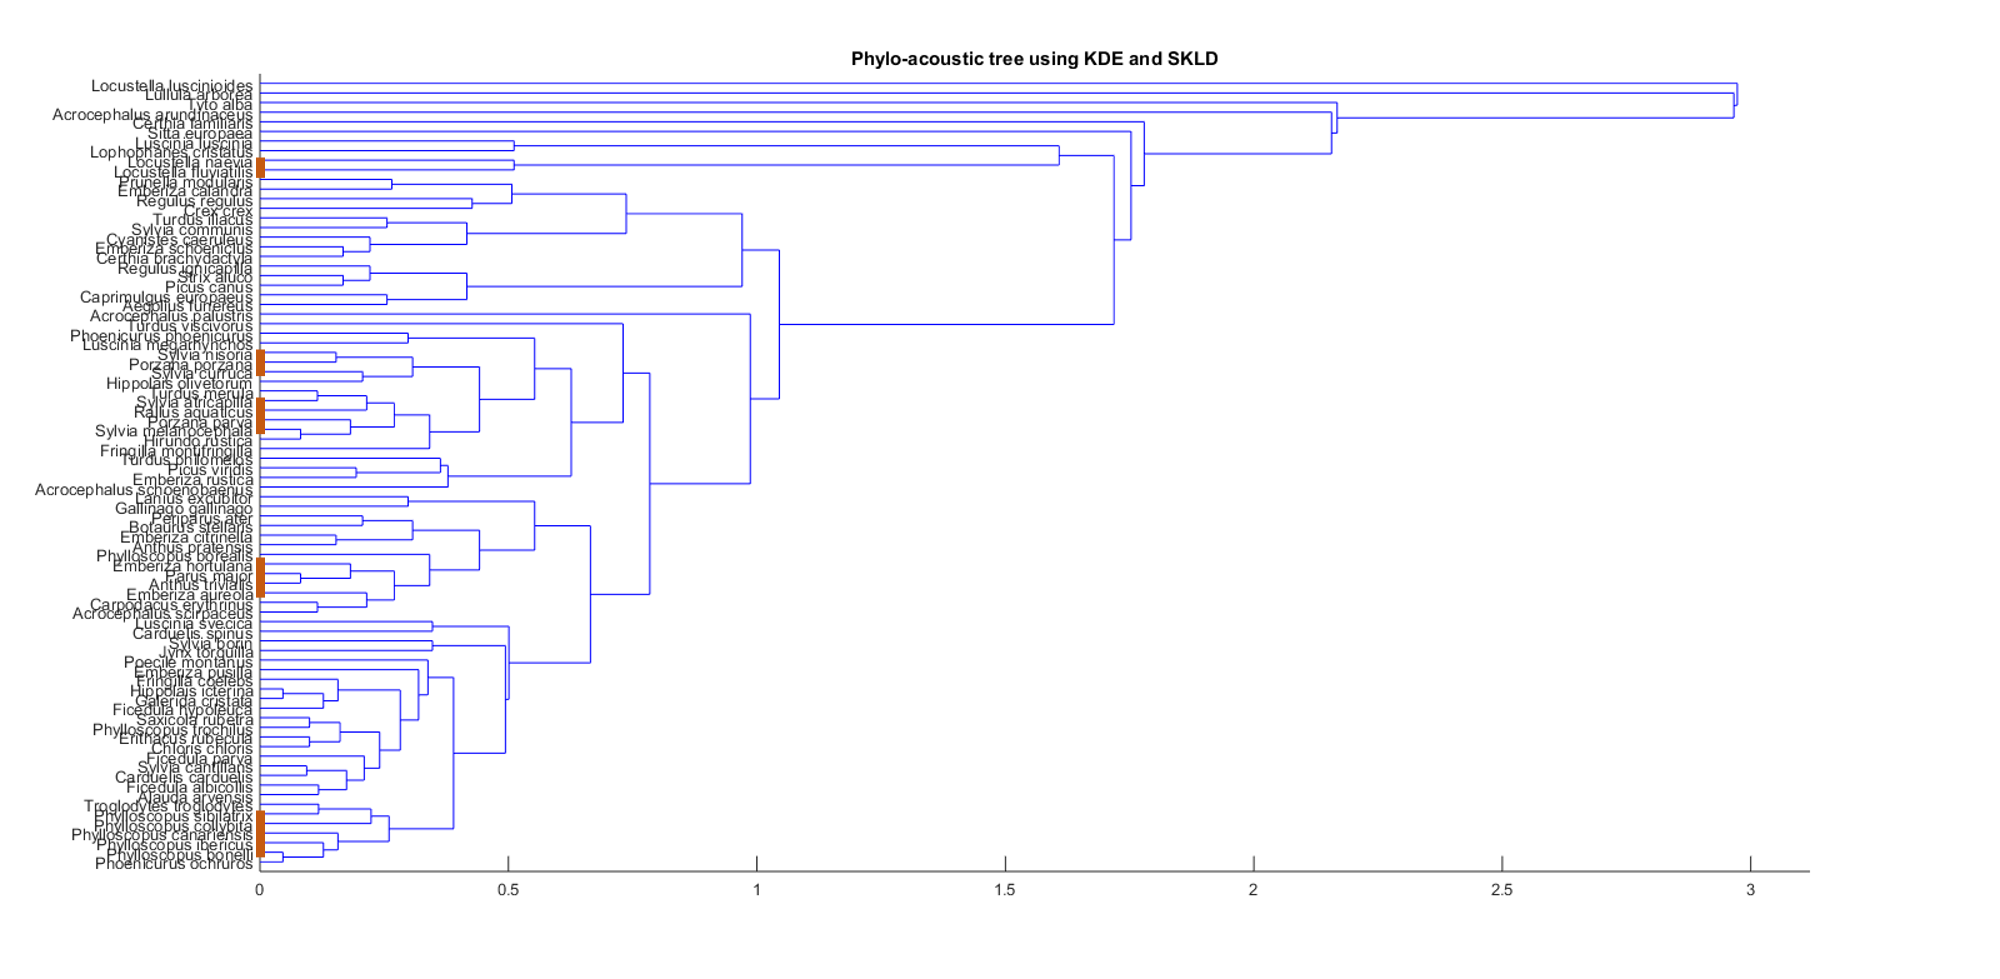
\includegraphics[width=\paperwidth]{kde_skld_2}}
    \caption{Phylo-acoustic tree generated using the Symmetric KL Divergence between pairs of non-parametric distributions generated using KDE.}
    \label{fig:kdeskld}
\end{sidewaysfigure}


\begin{sidewaysfigure}[ht]
\noindent\makebox[\textwidth]{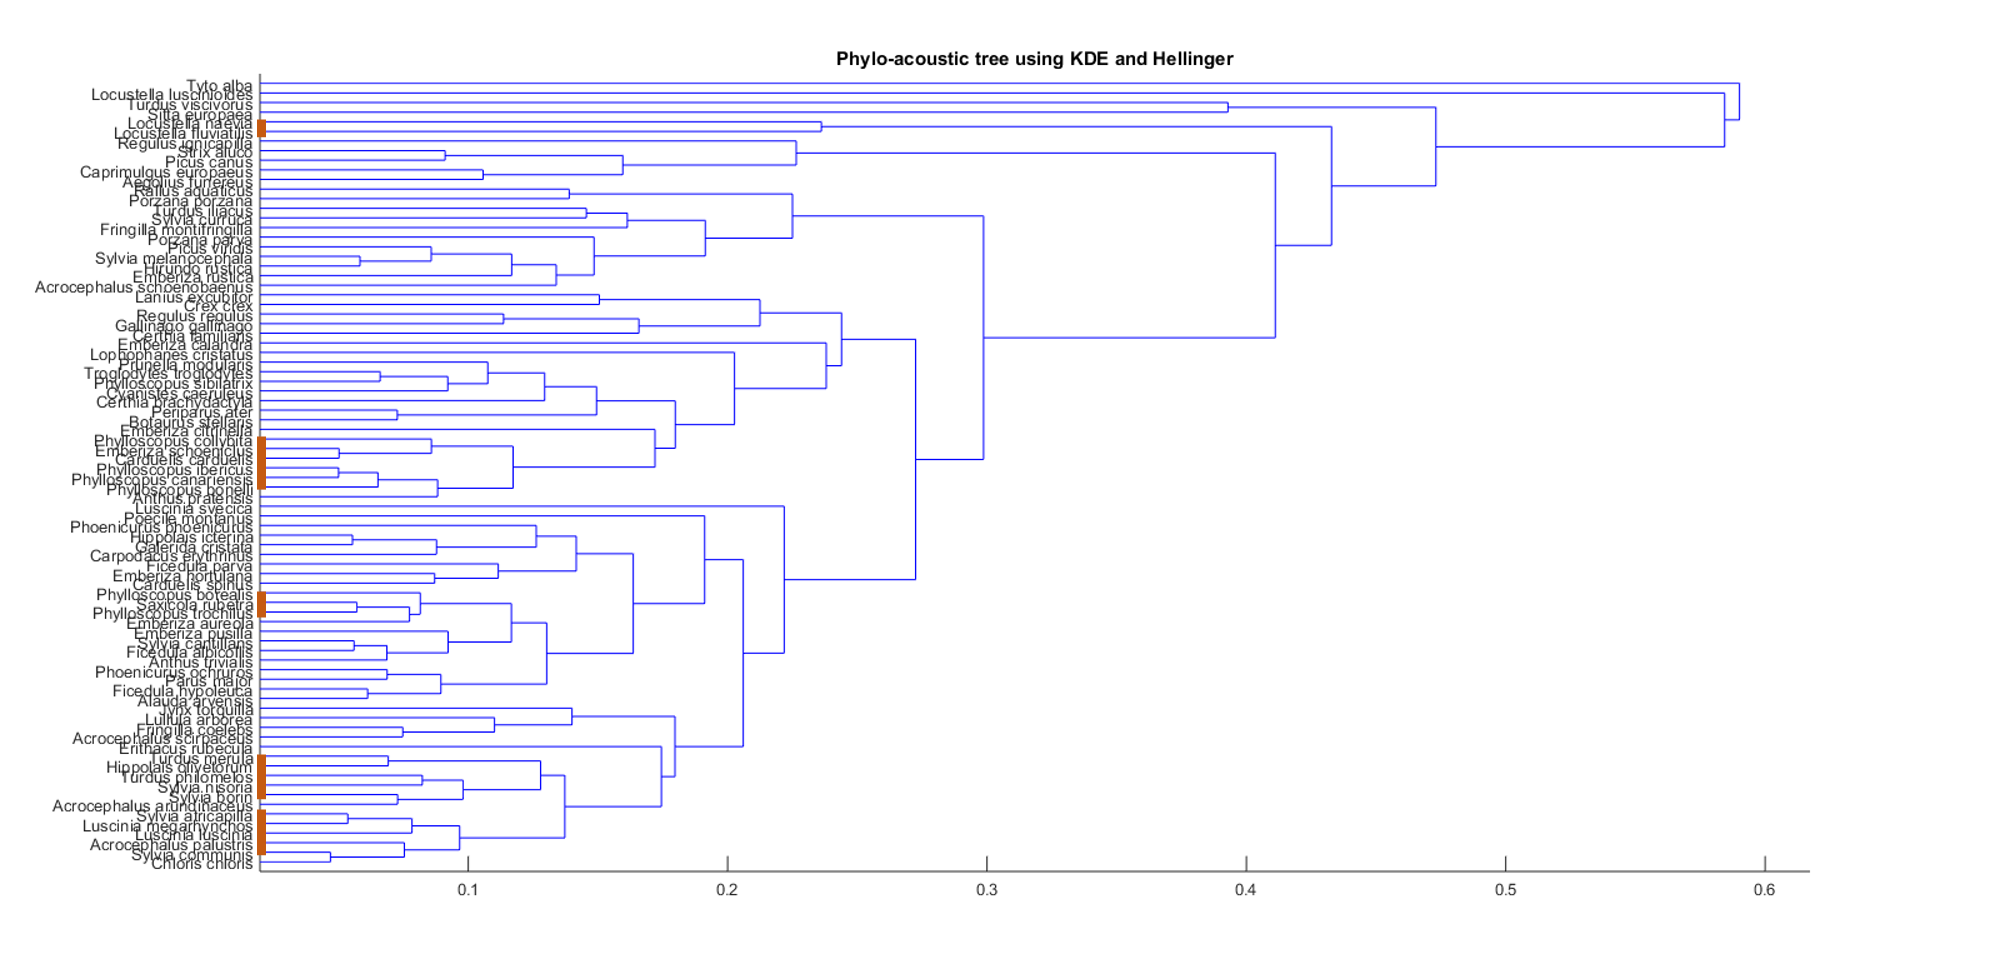
\includegraphics[width=\paperwidth]{kde_hellinger_2}}
    \caption{Phylo-acoustic tree generated using the Hellinger distance between pairs of non-parametric distributions generated using KDE.}
    \label{fig:kdehellinger}
\end{sidewaysfigure}


\begin{sidewaysfigure}[ht]
\noindent\makebox[\textwidth]{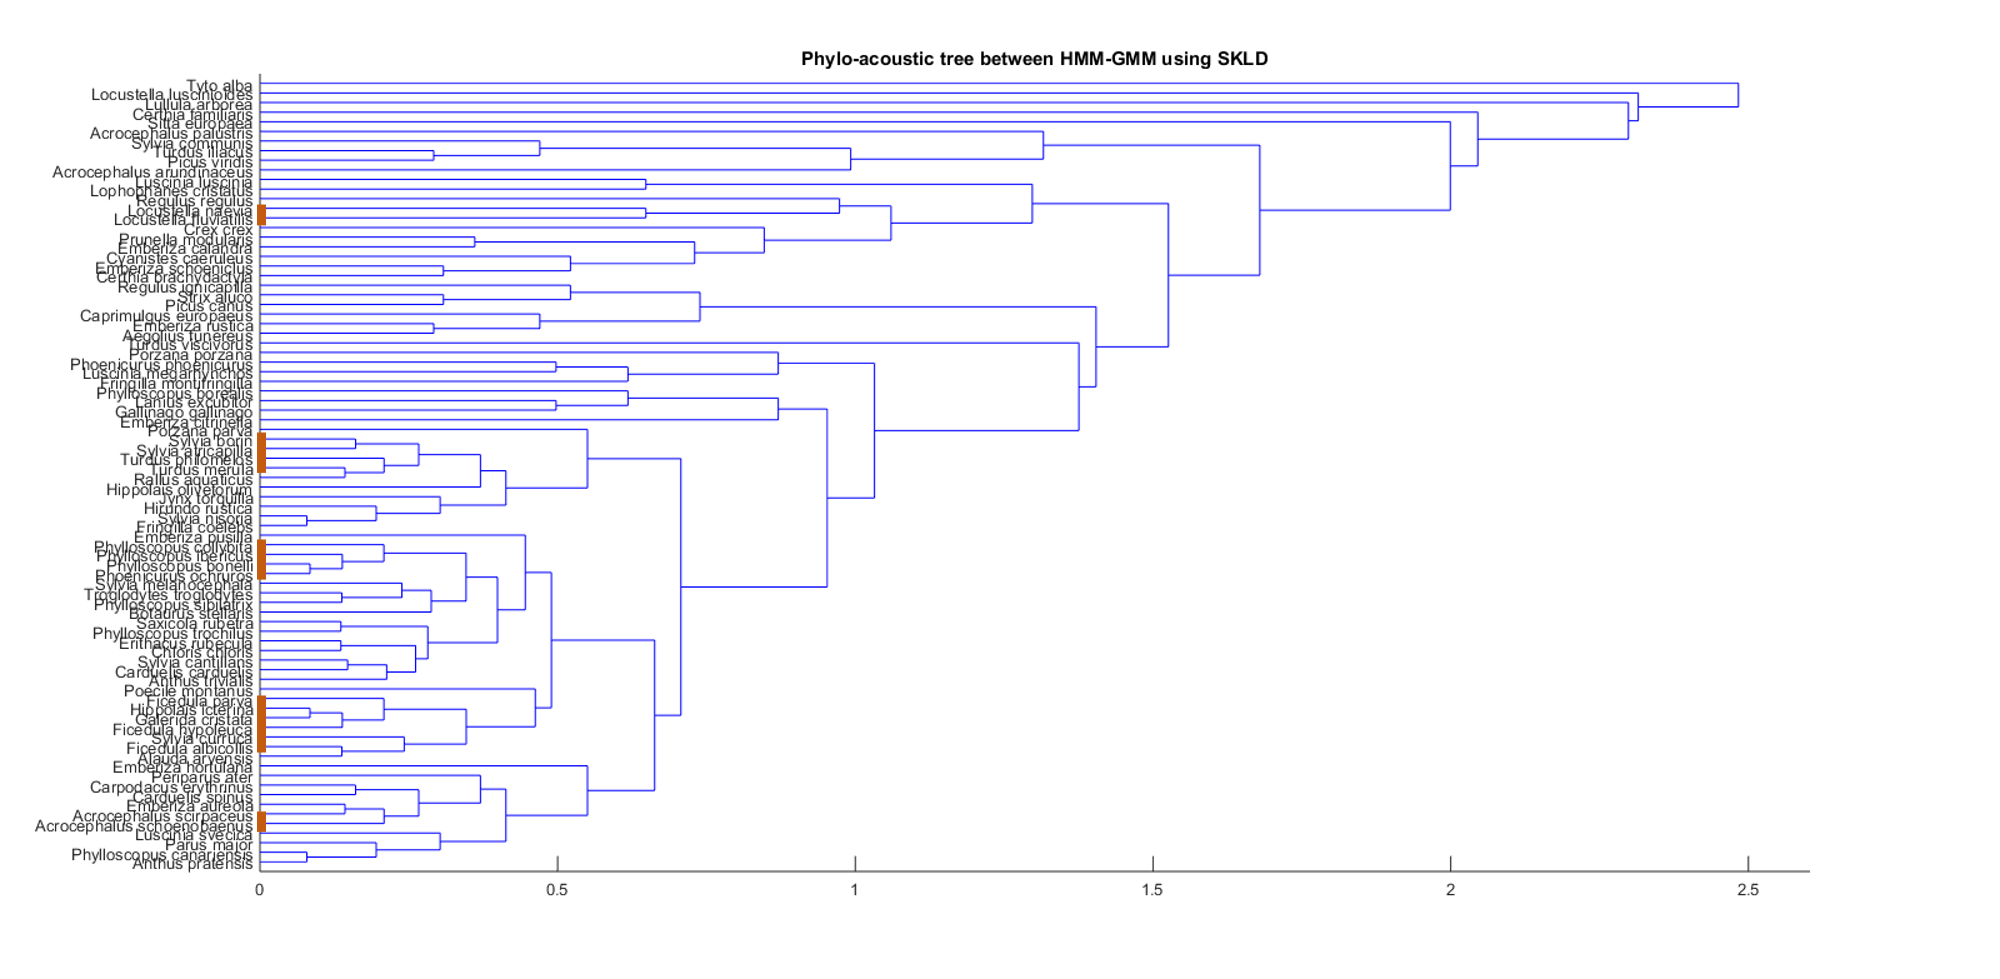
\includegraphics[width=\paperwidth]{gmm_skld_2}}
    %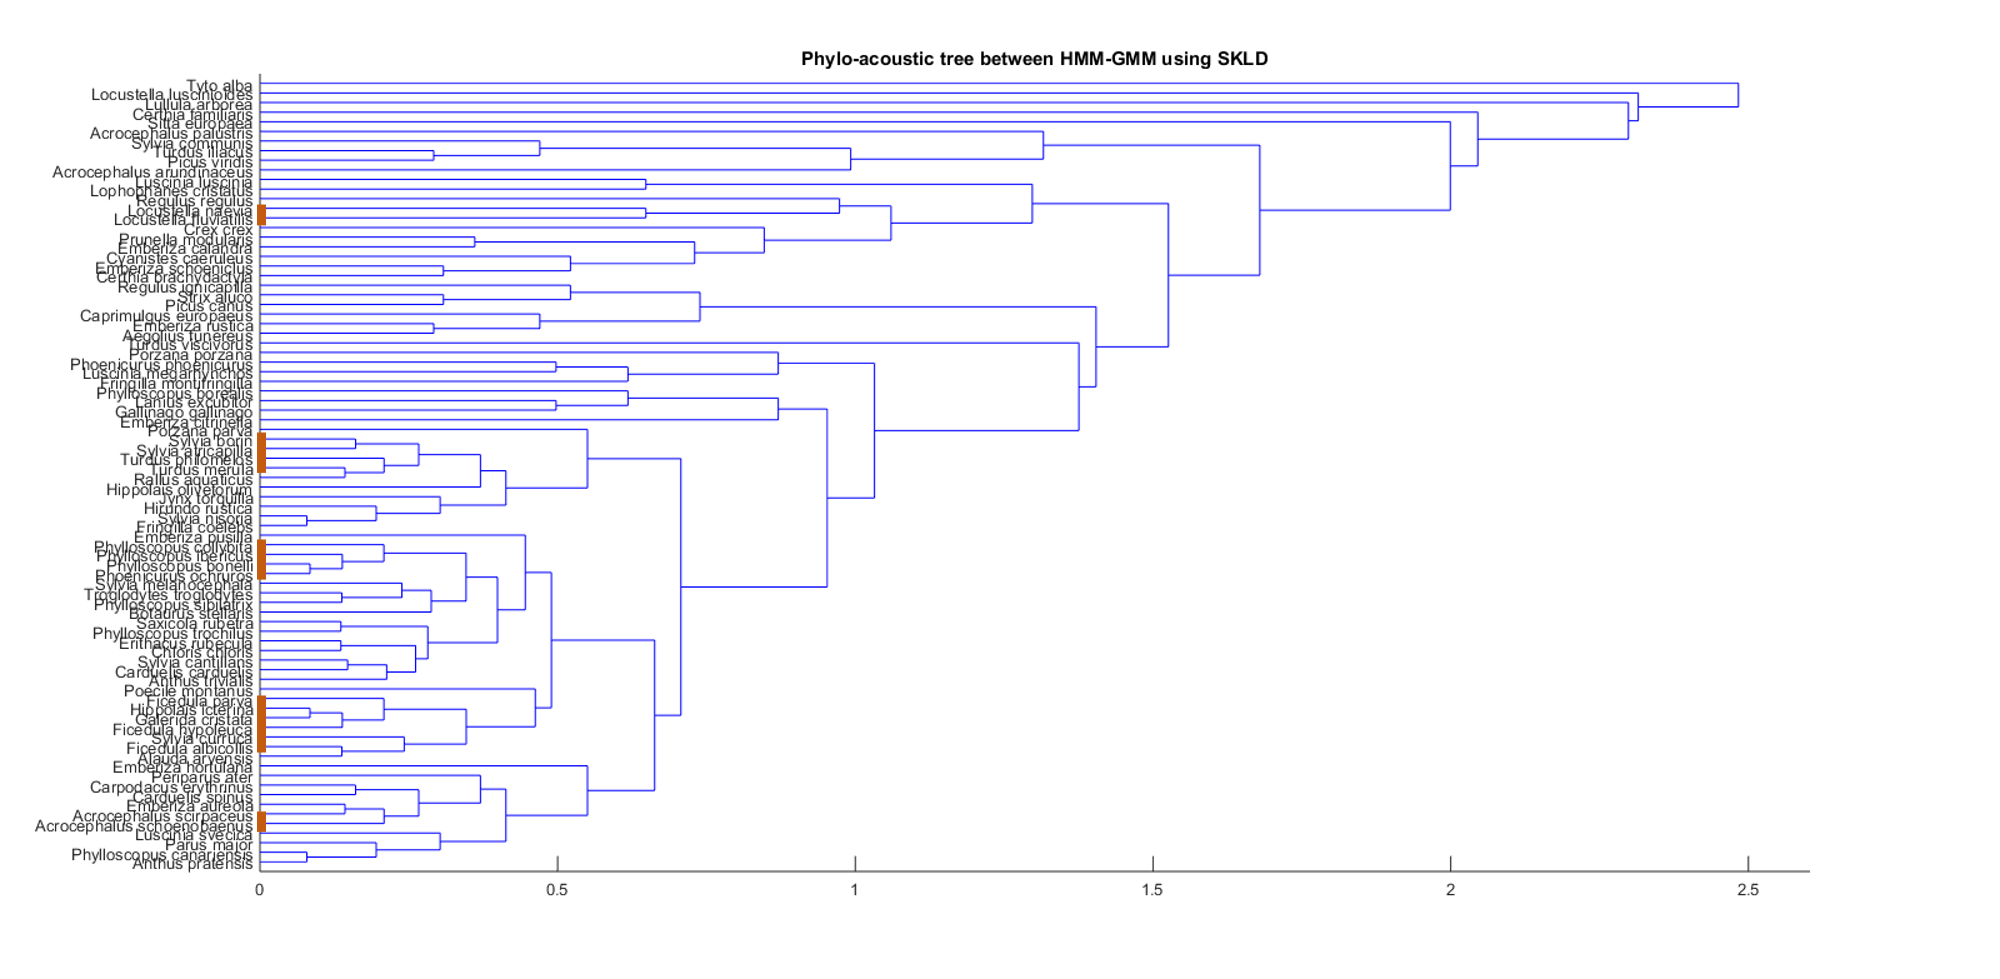
\includegraphics[width=\textwidth]{gmm_skld_2}
    \caption{Phylo-acoustic tree generated using the Symmetric KL-Divergence between pairs of emission models (GMMs) from HMMs.}
    \label{fig:gmmskld}
\end{sidewaysfigure}


\begin{sidewaysfigure}[ht]
\noindent\makebox[\textwidth]{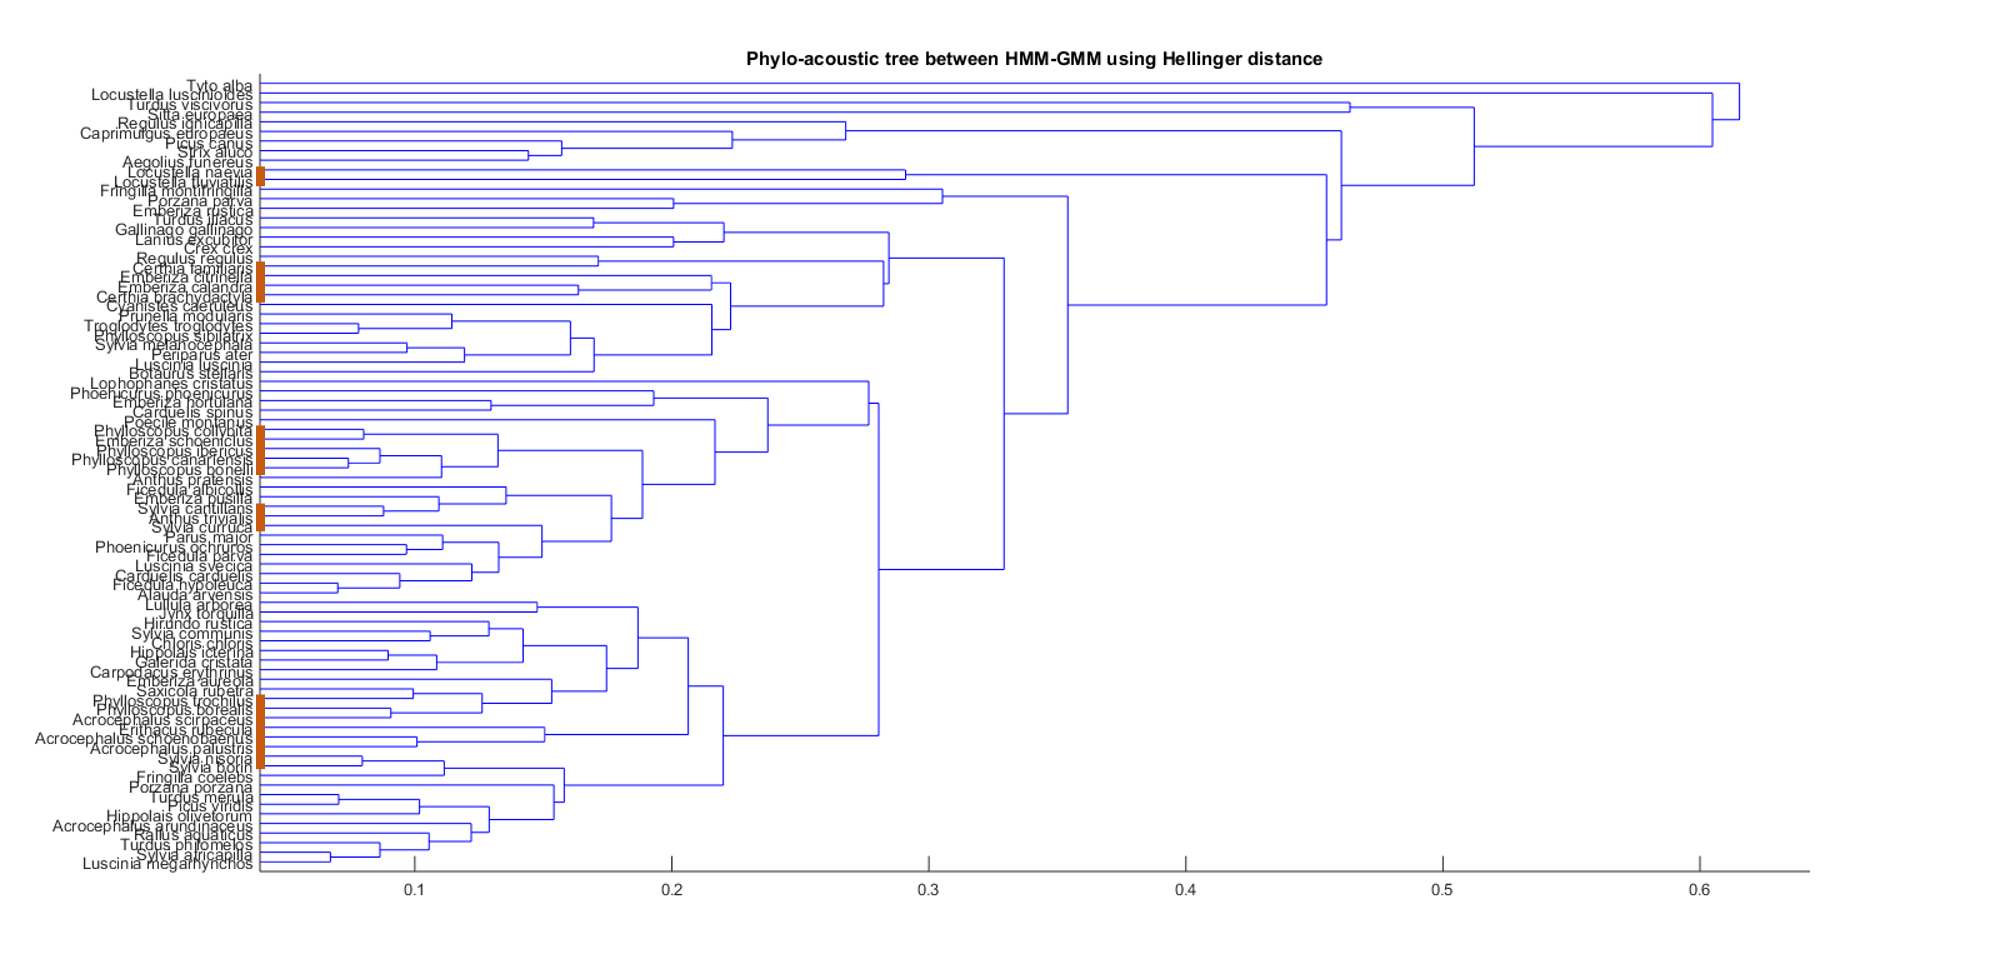
\includegraphics[width=\paperwidth]{gmm_hellinger_2}}
    \caption{Phylo-acoustic tree generated using the Hellinger distance between pairs of emission models (GMMs) from HMMs.}
    \label{fig:gmmhellinger}
\end{sidewaysfigure}


\begin{sidewaysfigure}[ht]
\noindent\makebox[\textwidth]{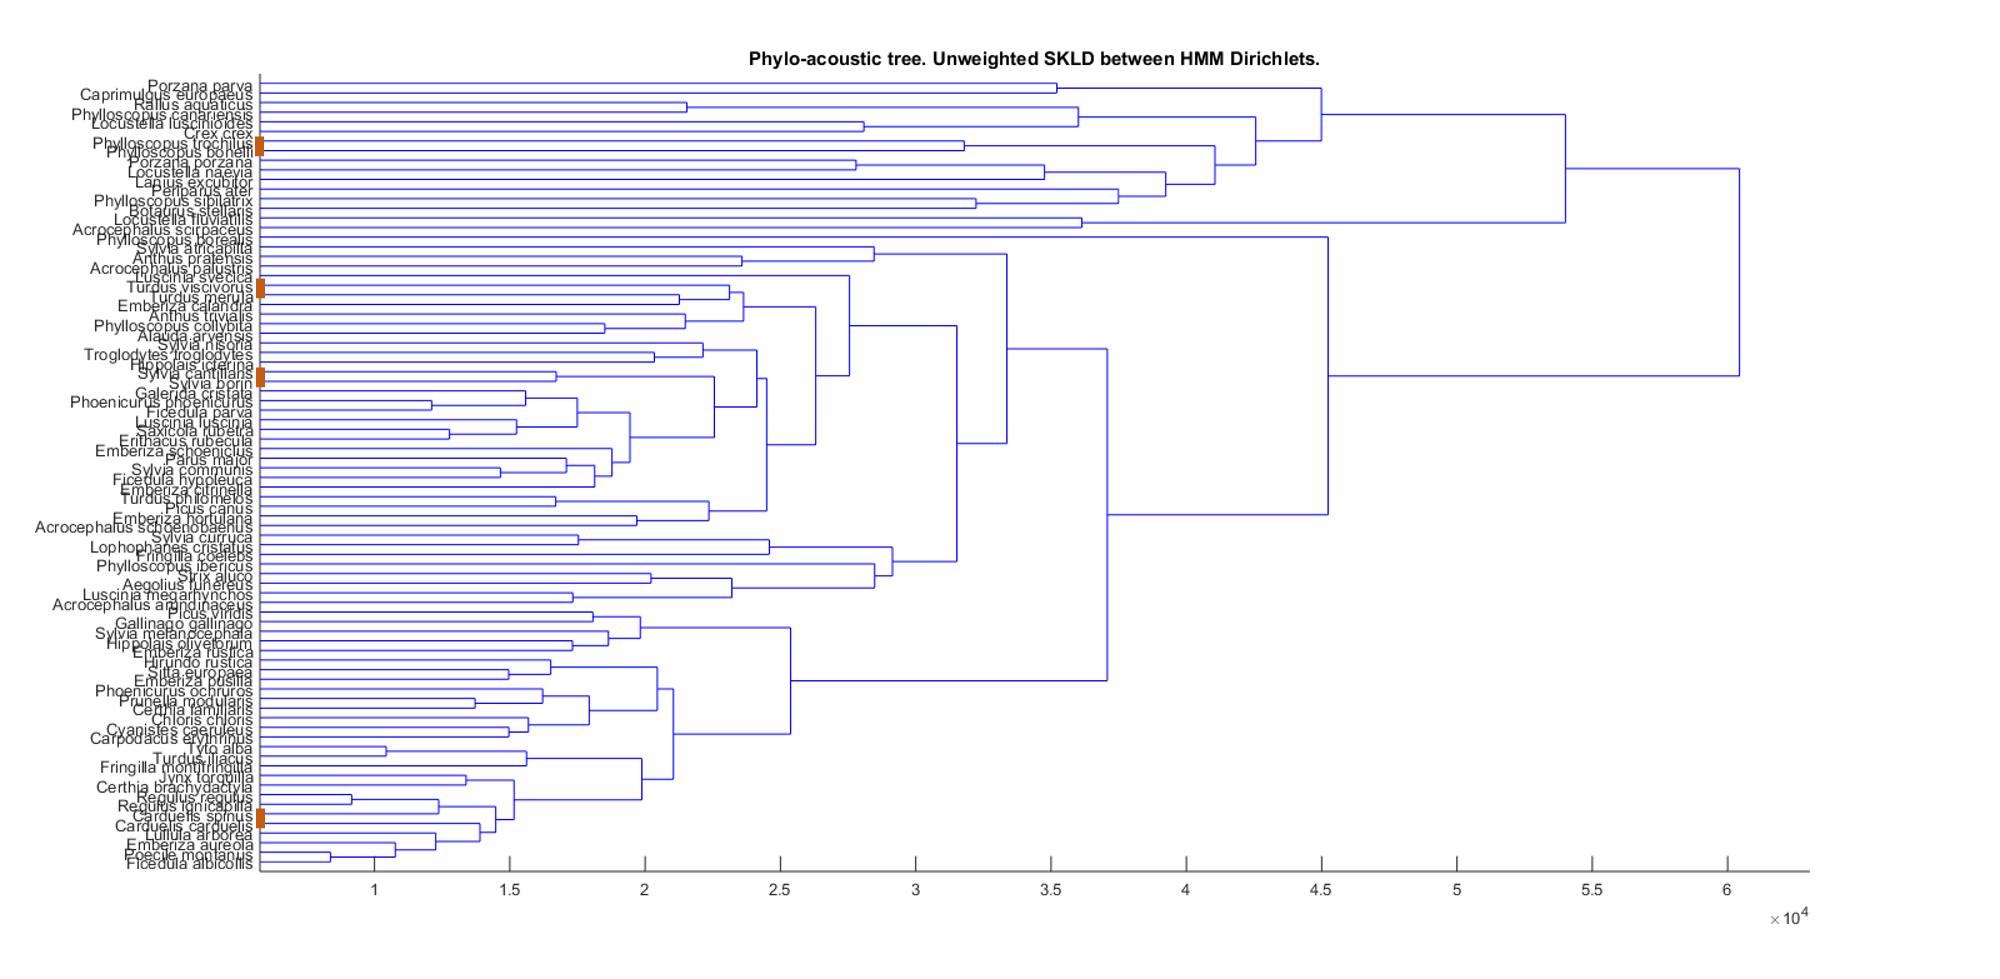
\includegraphics[width=\paperwidth]{dirichlet_unweighted_2}}
    \caption{Phylo-acoustic tree generated using the Symmetric KL-Divergence between pairs of transition models (Dirichlets) from HMMs.}
    \label{fig:hmmunweighted}
\end{sidewaysfigure}


\begin{sidewaysfigure}[ht]
\noindent\makebox[\textwidth]{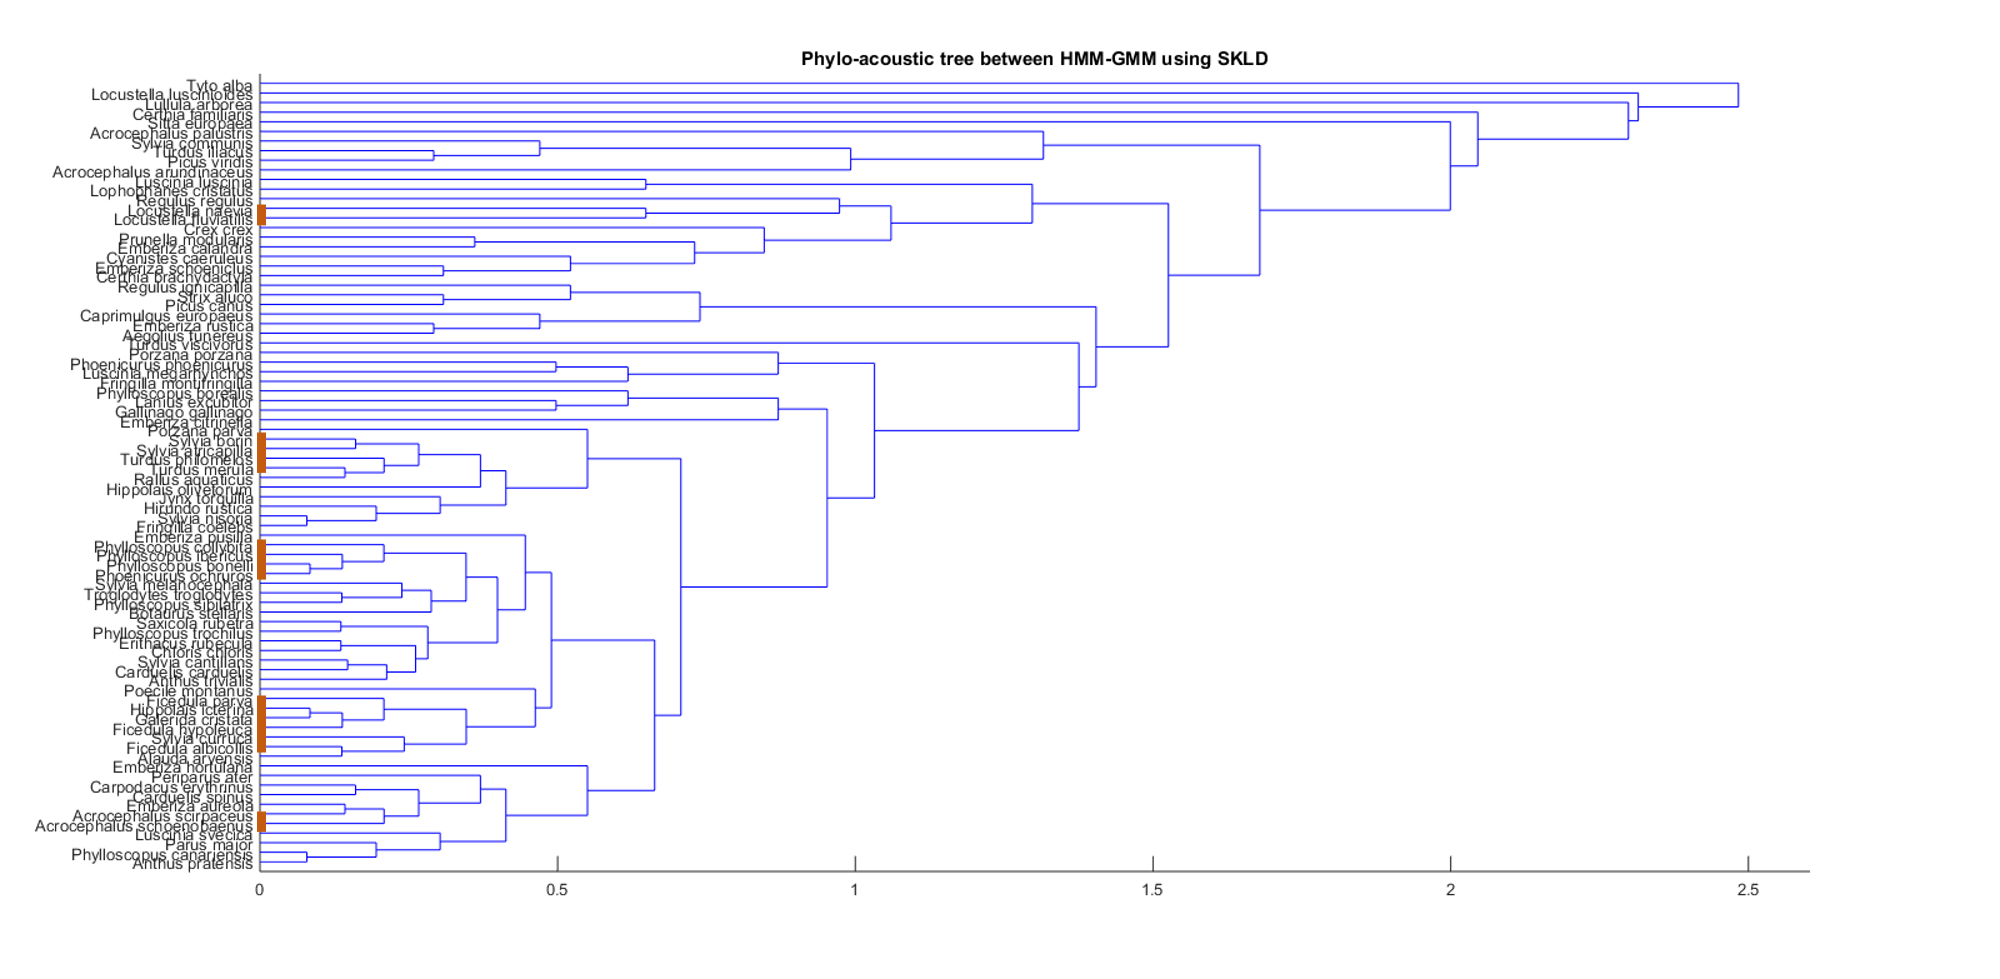
\includegraphics[width=\paperwidth]{gmm_skld_2}}
    \caption{Phylo-acoustic tree generated using the occupancy-weighted Symmetric KL-Divergence (see section \ref{subsection_hmmsim}) between pairs of transition models (Dirichlets) from HMMs.}
    \label{fig:hmmweighted}
\end{sidewaysfigure}



\begin{sidewaysfigure}[ht]
\noindent\makebox[\textwidth]{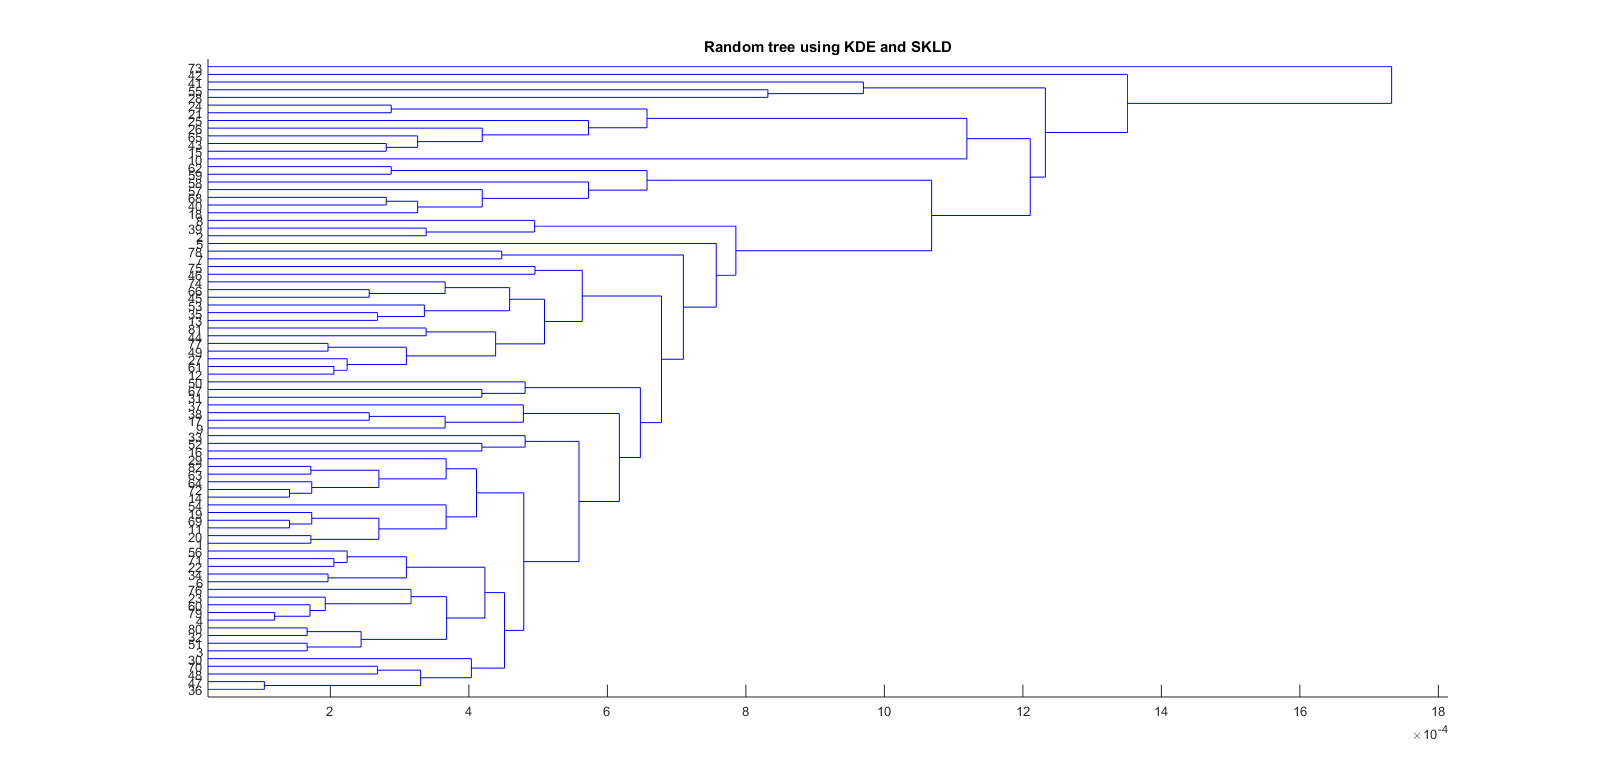
\includegraphics[width=\paperwidth]{random_kde_skld}}
    \caption{Random phylo-acoustic tree generated using the Symmetric KL Divergence between pairs of non-parametric distributions generated using KDE.}
    \label{fig:rkdeskld}
\end{sidewaysfigure}


\begin{sidewaysfigure}[ht]
\noindent\makebox[\textwidth]{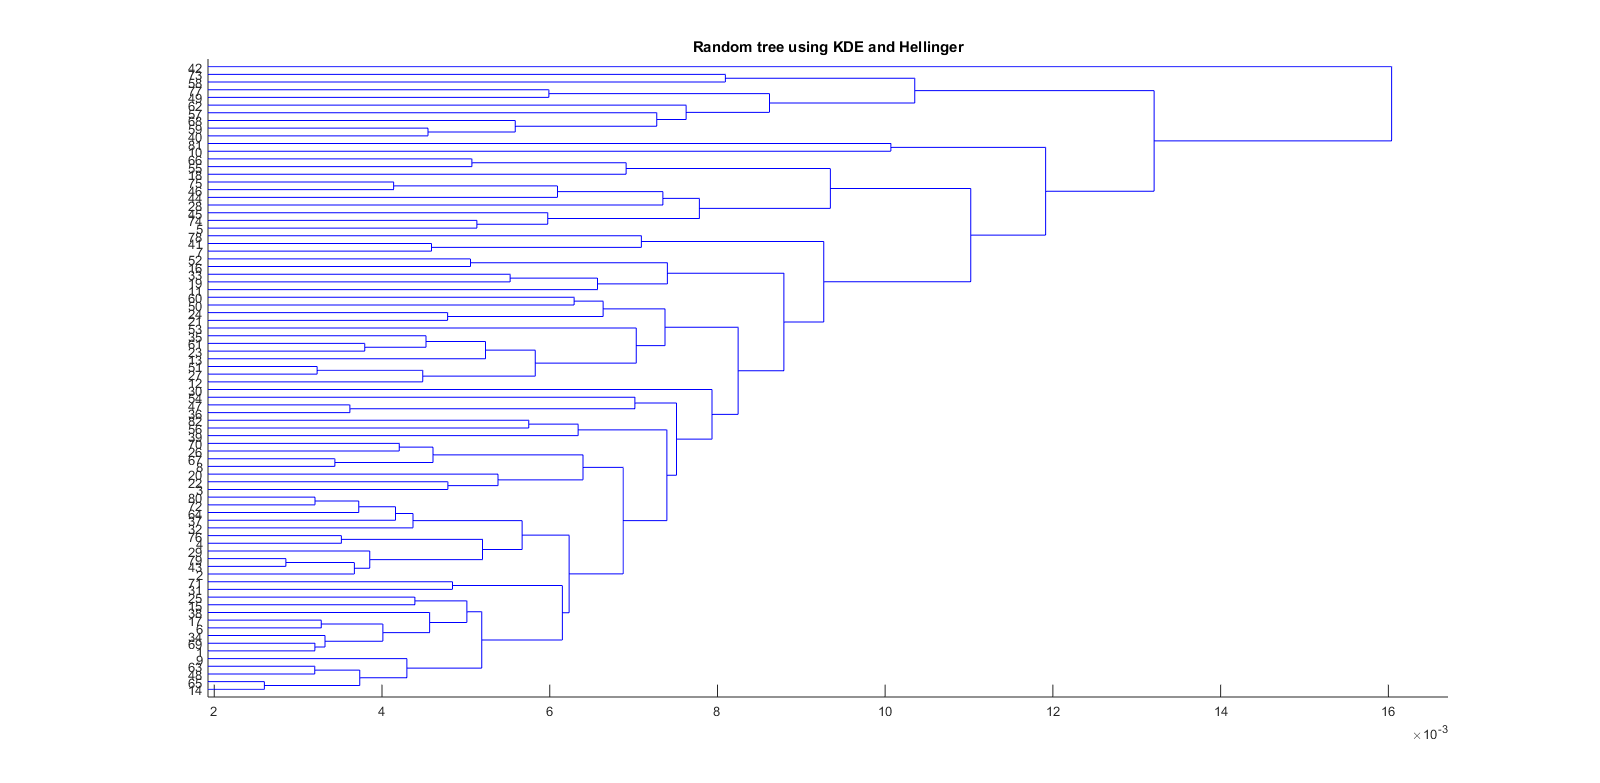
\includegraphics[width=\paperwidth]{random_kde_hellinger}}
    \caption{Random phylo-acoustic tree generated using the Hellinger distance between pairs of non-parametric distributions generated using KDE.}
    \label{fig:rkdehellinger}
\end{sidewaysfigure}


\begin{sidewaysfigure}[ht]
\noindent\makebox[\textwidth]{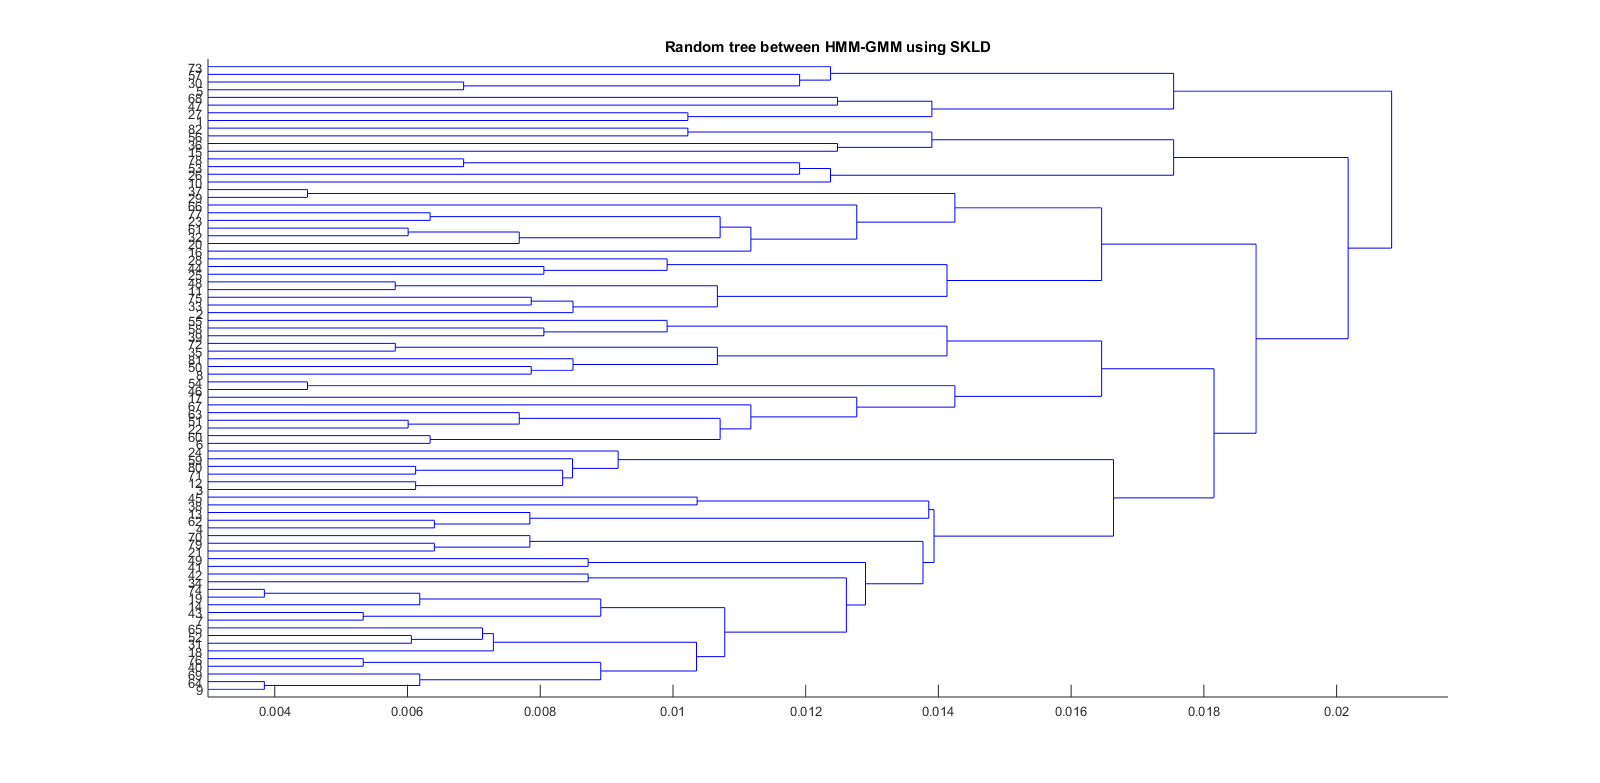
\includegraphics[width=\paperwidth]{random_gmm_skld}}
    \caption{Random phylo-acoustic tree generated using the Symmetric KL-Divergence between pairs of emission models (GMMs) from HMMs.}
    \label{fig:rgmmskld}
\end{sidewaysfigure}


\begin{sidewaysfigure}[ht]
\noindent\makebox[\textwidth]{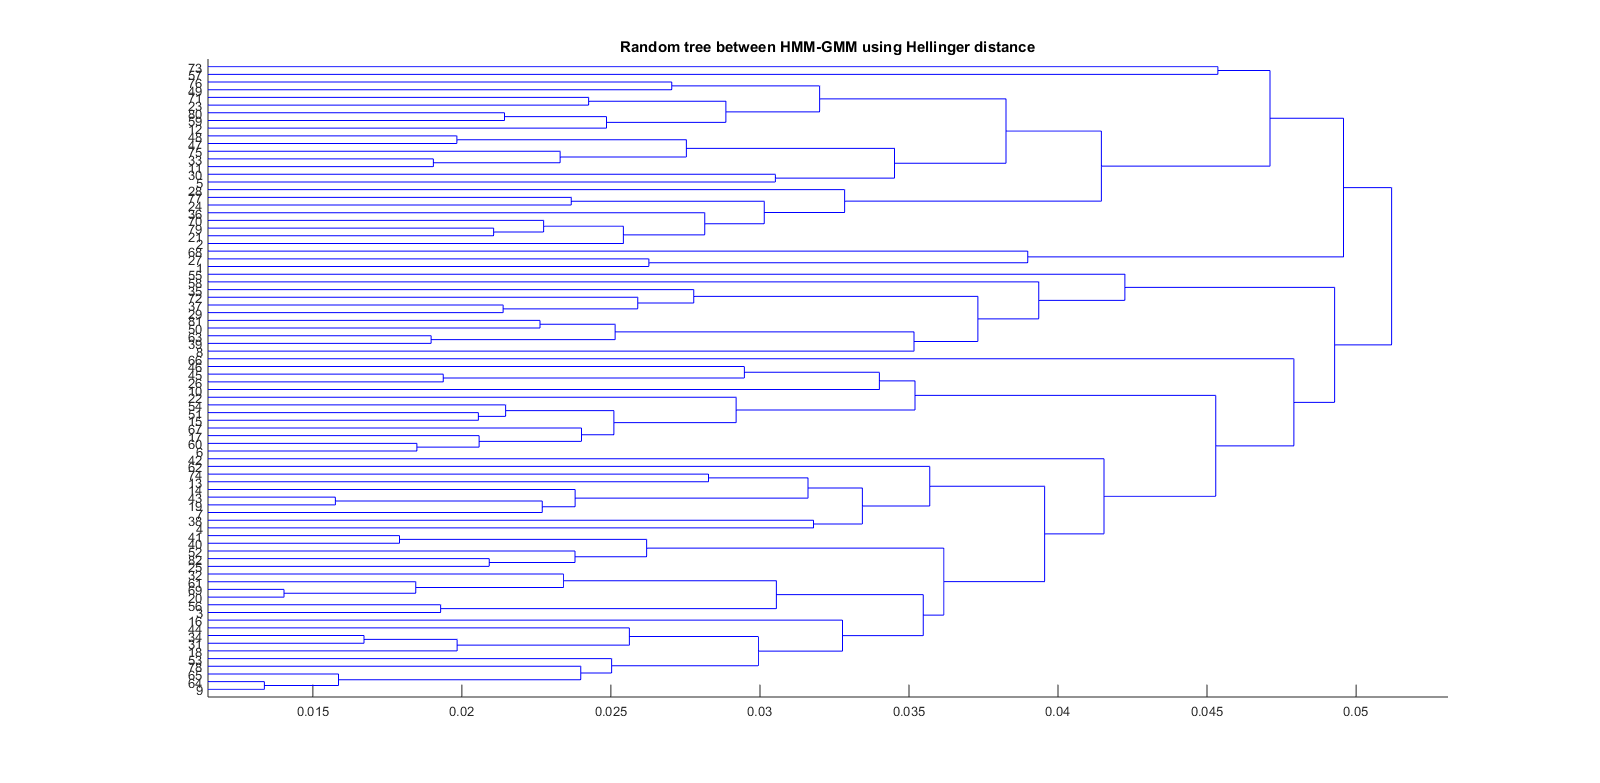
\includegraphics[width=\paperwidth]{random_gmm_hellinger}}
    \caption{Random phylo-acoustic tree generated using the Hellinger distance between pairs of emission models (GMMs) from HMMs.}
    \label{fig:rgmmhellinger}
\end{sidewaysfigure}


\begin{sidewaysfigure}[ht]
\noindent\makebox[\textwidth]{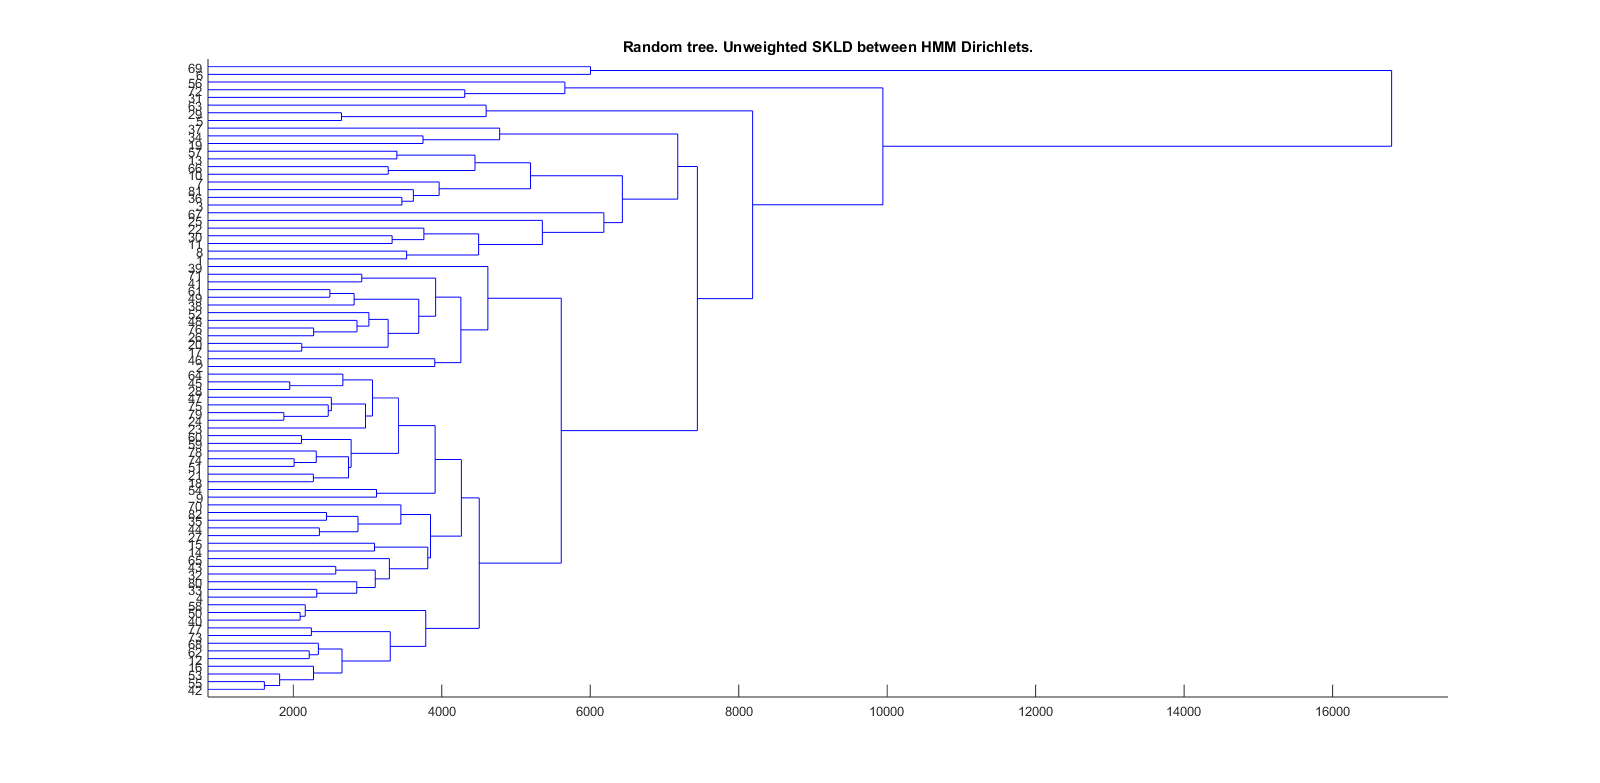
\includegraphics[width=\paperwidth]{random_dirichlet_unweighted}}
    \caption{Random phylo-acoustic tree generated using the Symmetric KL-Divergence between pairs of transition models (Dirichlets) from HMMs.}
    \label{fig:rhmmunweighted}
\end{sidewaysfigure}


\begin{sidewaysfigure}[ht]
\noindent\makebox[\textwidth]{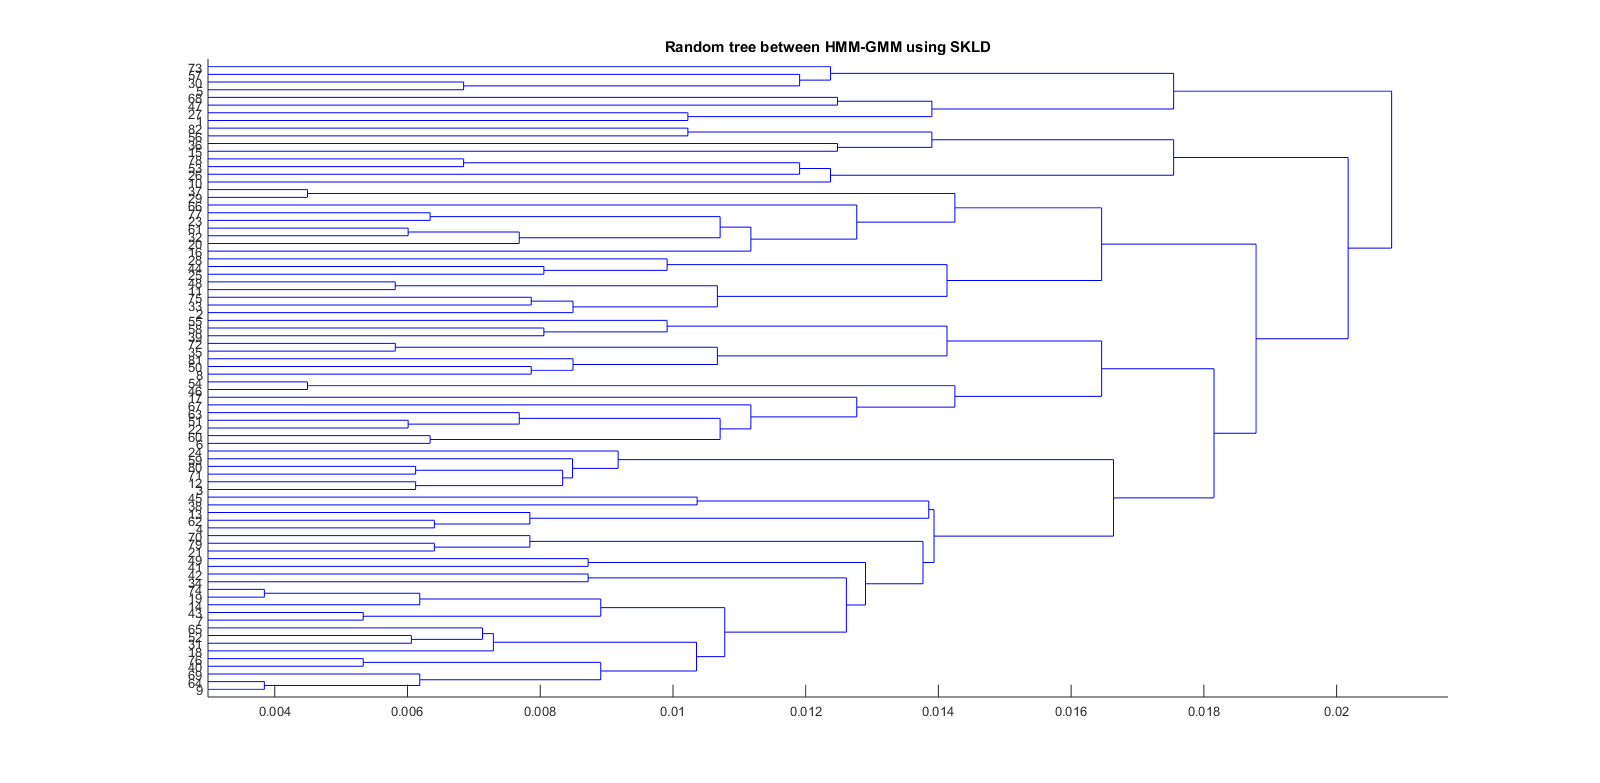
\includegraphics[width=\paperwidth]{random_gmm_skld}}
    \caption{Random phylo-acoustic tree generated using the occupancy-weighted Symmetric KL-Divergence (see section \ref{subsection_hmmsim}) between pairs of transition models (Dirichlets) from HMMs.}
    \label{fig:rhmmweighted}
\end{sidewaysfigure}

\begin{figure}[t]
\centering
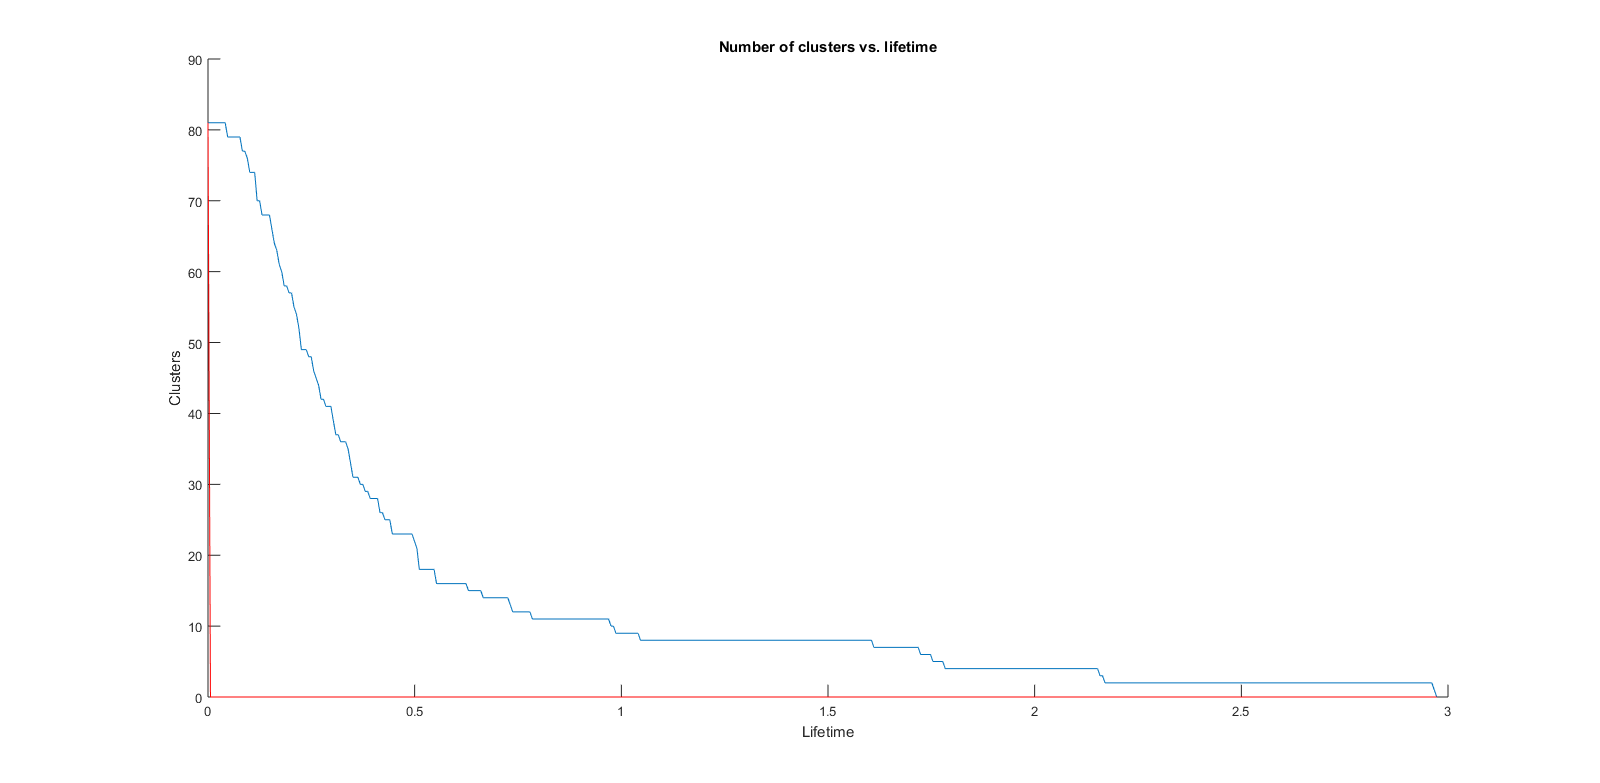
\includegraphics[width=\textwidth]{lifetime_kde_skld}
\caption{Lifetime vs. number of clusters using the Symmetric KL Divergence between non-parametric distributions obtained via KDE.}
\label{fig_lt_kde_skld}
\end{figure}

\begin{figure}[t]
\centering
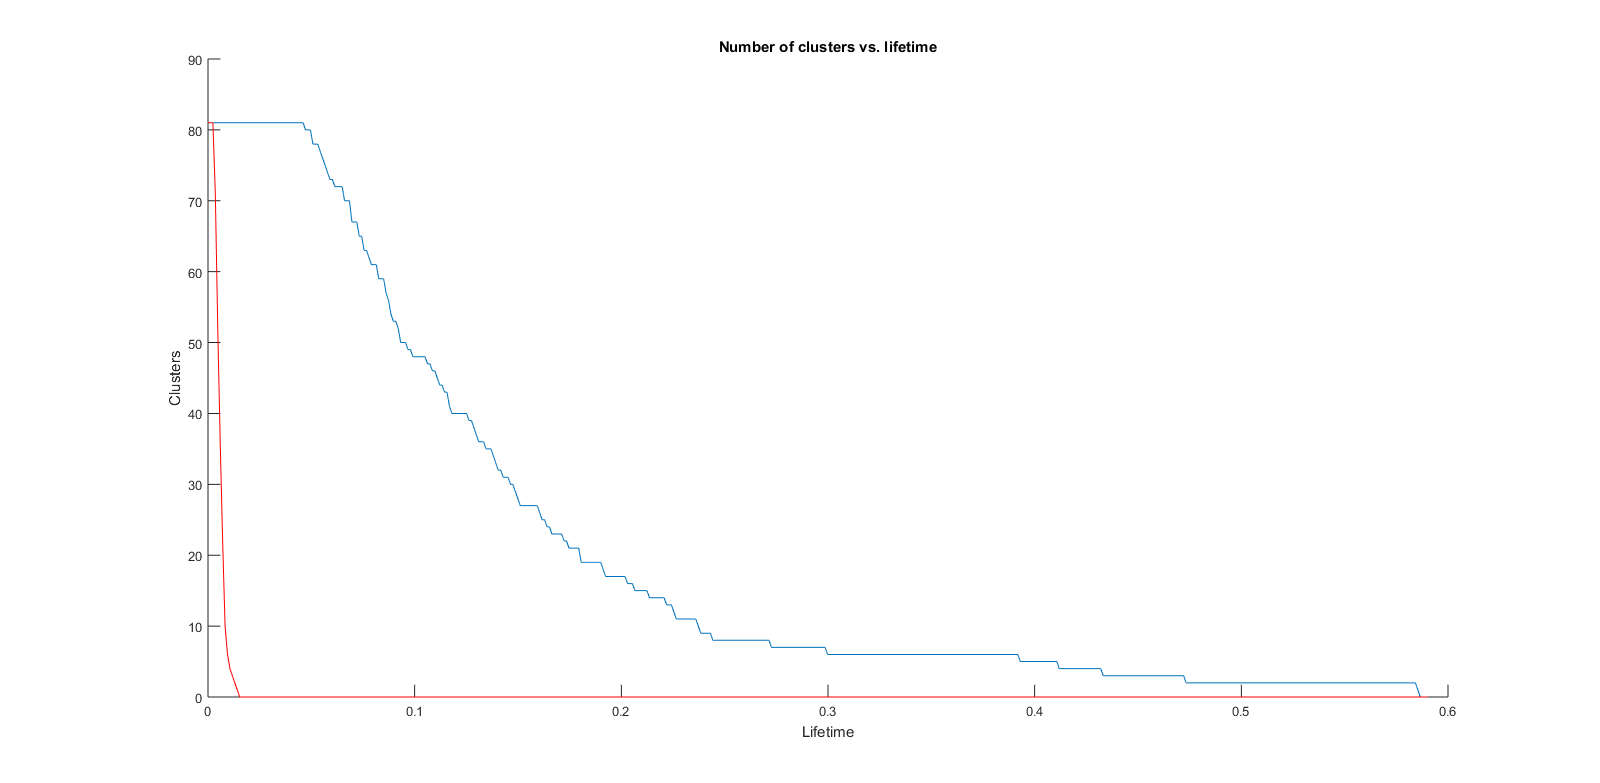
\includegraphics[width=\textwidth]{lifetime_kde_hellinger}
\caption{Lifetime vs. number of clusters using the Hellinger distance between non-parametric distributions obtained via KDE.}
\label{fig_lt_kde_hellinger}
\end{figure}

\begin{figure}[t]
\centering
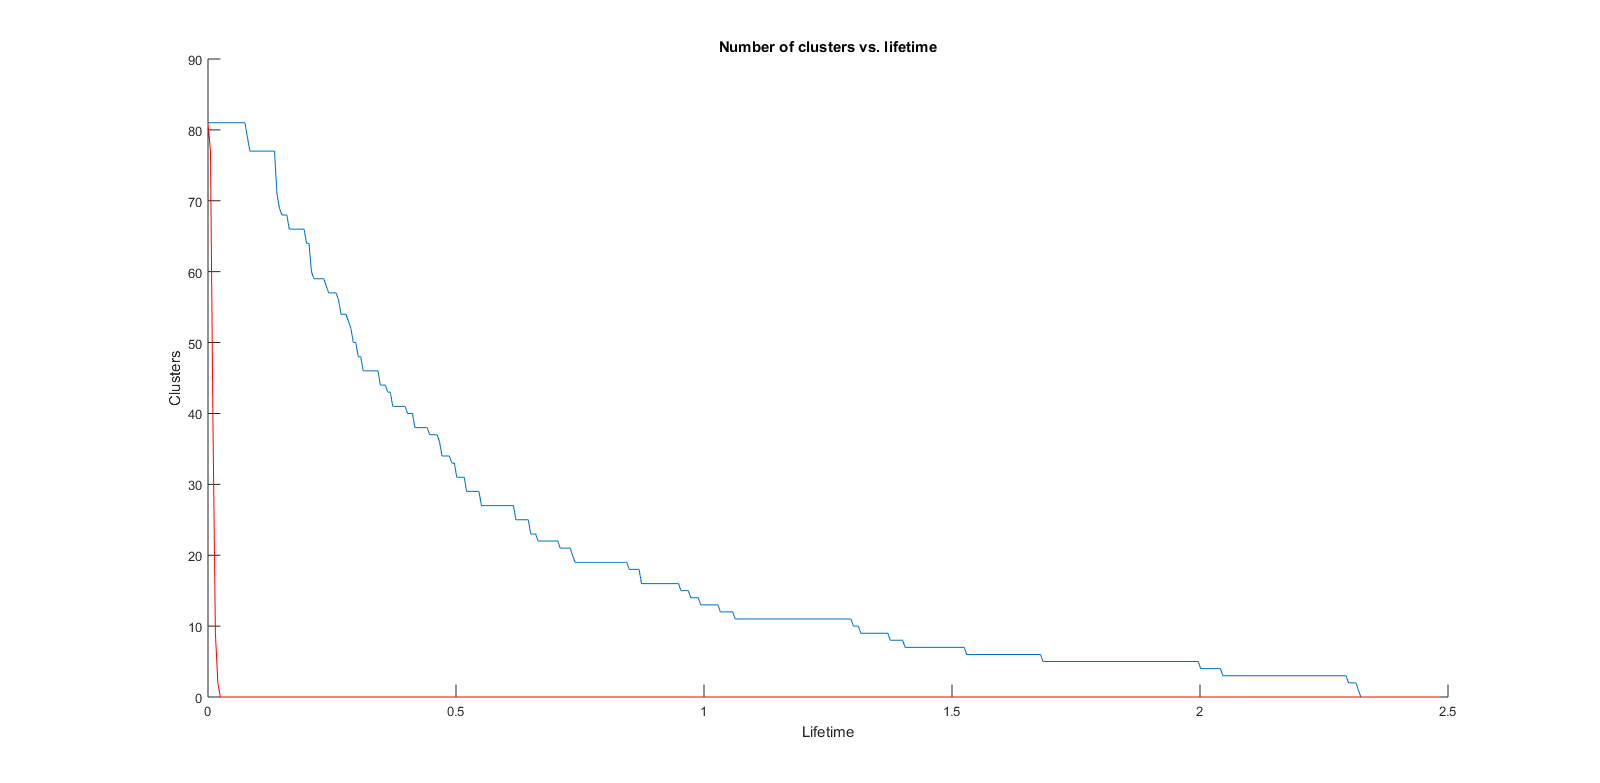
\includegraphics[width=\textwidth]{lifetime_gmm_skld}
\caption{Lifetime vs. number of clusters using the Symmetric KL Divergence between HMM emission models (GMMs).}
\label{fig_lt_gmm_skld}
\end{figure}

\begin{figure}[t]
\centering
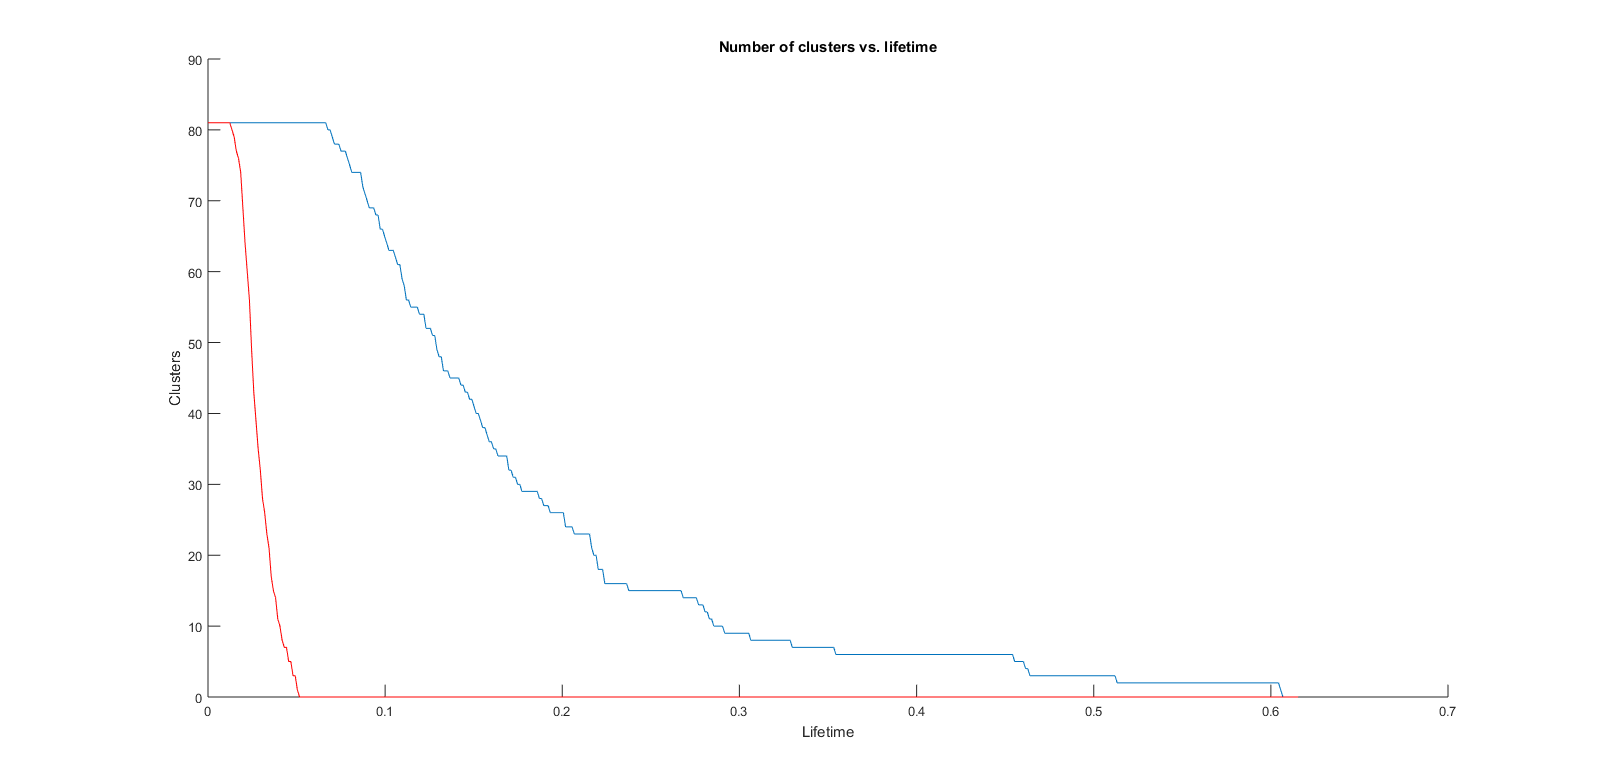
\includegraphics[width=\textwidth]{lifetime_gmm_hellinger}
\caption{Lifetime vs. number of clusters using the Hellinger distance between HMM emission models (GMMs).}
\label{fig_lt_gmm_hellinger}
\end{figure}

\begin{figure}[t]
\centering
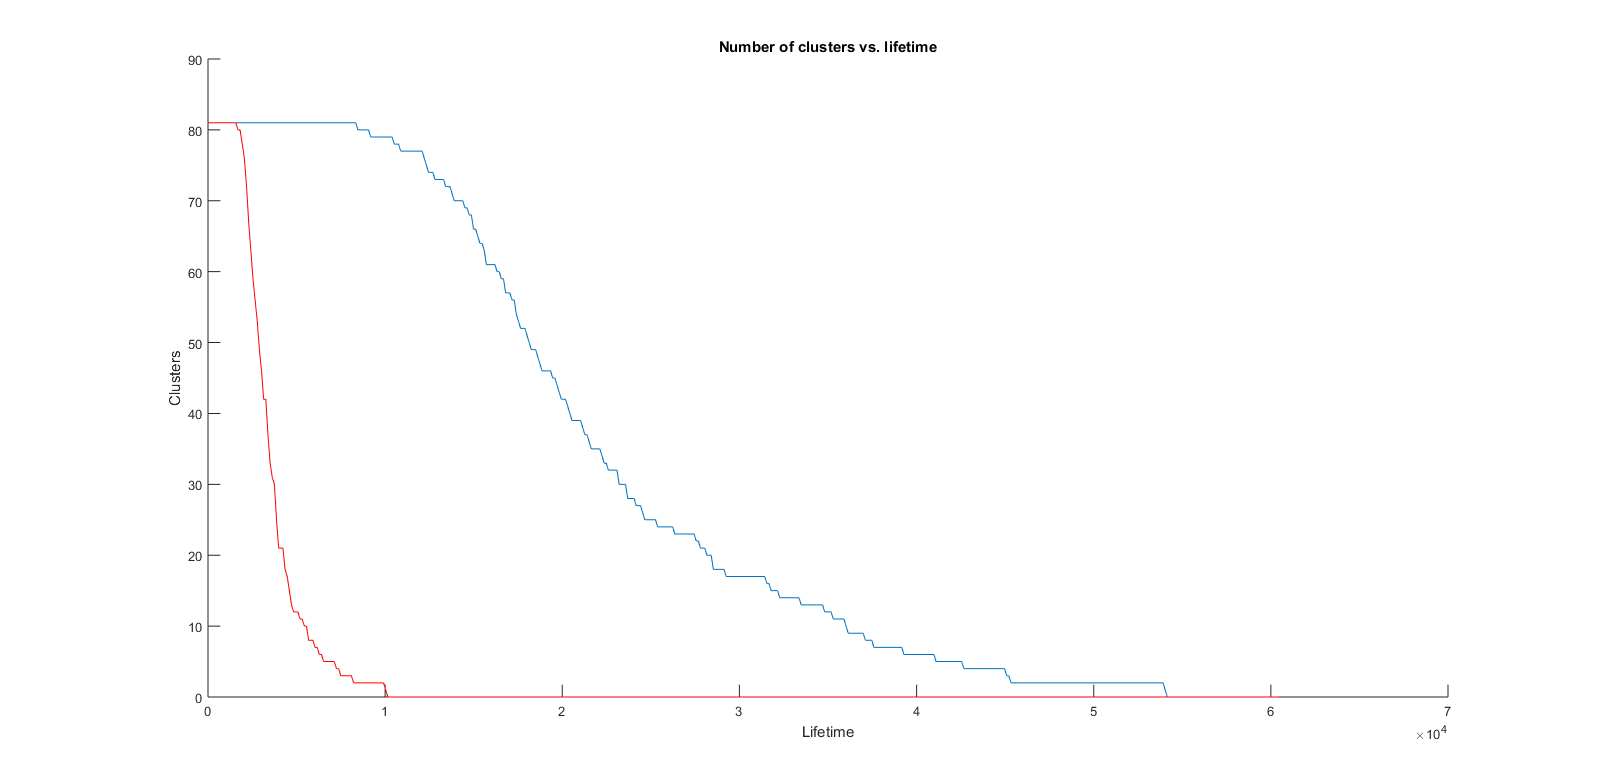
\includegraphics[width=\textwidth]{lifetime_dirichlet_unweighted}
\caption{Lifetime vs. number of clusters using the Dirichlet distance between HMMs.}
\label{fig_lt_du}
\end{figure}

\begin{figure}[t]
\centering
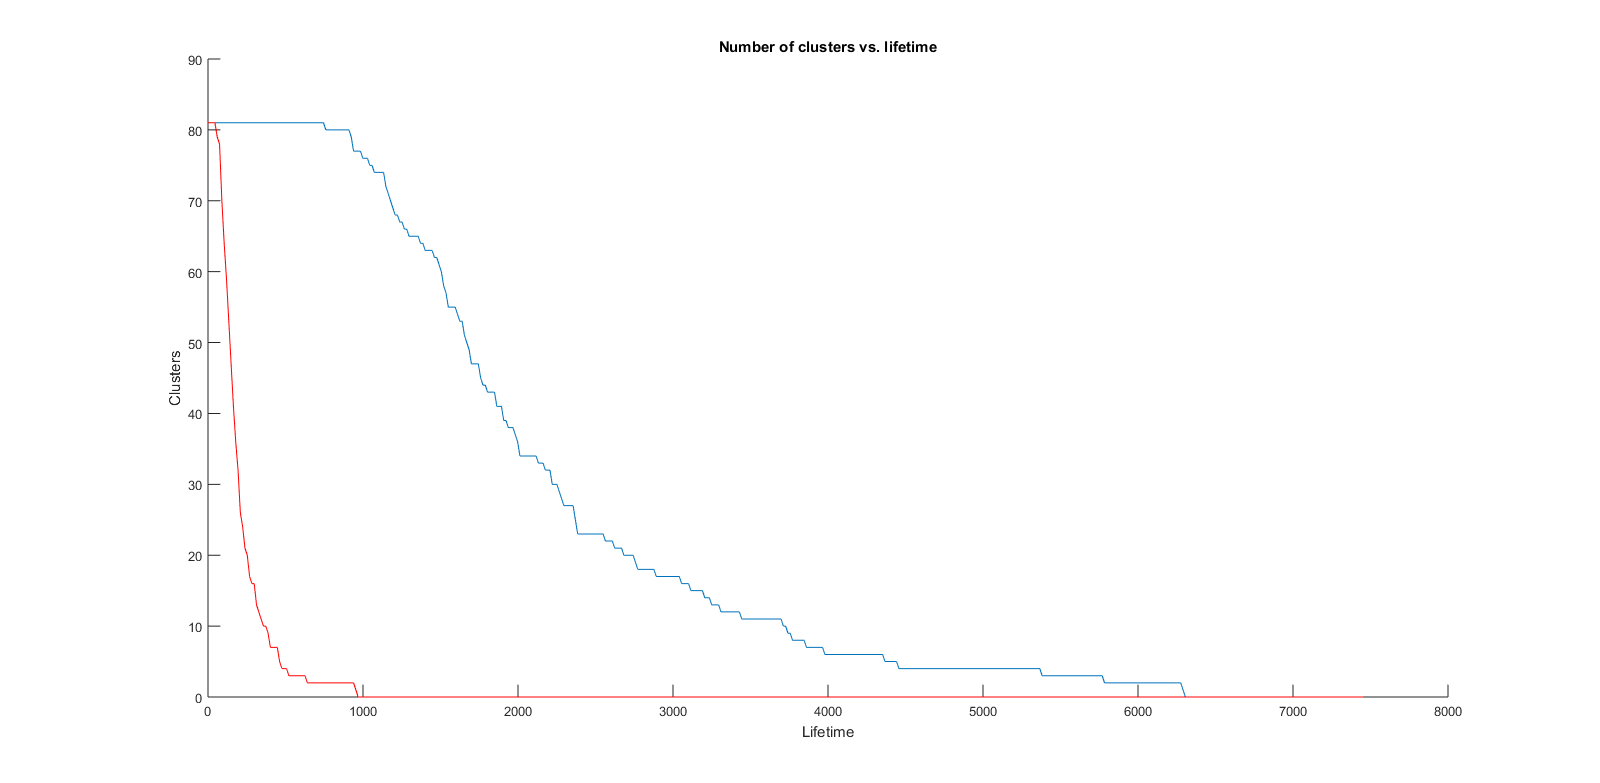
\includegraphics[width=\textwidth]{lifetimedirichlet_occupancy}
\caption{Lifetime vs. number of clusters using the Occupancy-weighted Dirichlet distance between HMMs.}
\label{fig_lt_occ}
\end{figure}   
\end{document}